% Define document class
\documentclass[twocolumn]{aastex631}
\usepackage{showyourwork}
\usepackage[ruled,vlined,linesnumbered]{algorithm2e}
\usepackage{algorithmic}
\usepackage{color}
%\usepackage[dvipsnames]{xcolor}

\definecolor{rb4}{HTML}{27408B}
\newcommand{\kw}[1]{{\color{rb4}[KW: #1 ]}}
\definecolor{pyRed}{RGB}{214, 39, 40}
\newcommand{\te}[1]{\textbf{\color{pyRed}(TE: #1)}}
\newcommand{\mi}[1]{\textsf{\color{teal}[\textbf{MI:} #1]}}

\newcommand{\flatiron}{\affiliation{Center for Computational Astrophysics,
Flatiron Institute, New York, NY 10010, USA}}
\newcommand{\jhu}{\affiliation{William H. Miller III Department of Physics and Astronomy, Johns Hopkins University, Baltimore, Maryland 21218, USA}}

\SetKwInput{Parameters}{Parameters}
\SetKwInput{Variables}{Variables}

% Begin!
\begin{document}

% Title
\title{Fast  gravitational wave parameter estimation with no-compromise}
% Title Options
% \title{Ripples in the Flow: \\ Fast, General Parameter Estimation with Normalizing Flows and Differentiable Waveforms}

% Author list
\author{Kaze W. K. Wong}
\email{kwong@flatironinstitute.org}
\flatiron

\author{Maximiliano Isi}
\flatiron

\author{Thomas D. P. Edwards}
\jhu

% Abstract with filler text
\begin{abstract}
We present a lightweight, flexible, and high-performance framework for inferring
the properties of gravitational-wave events. By combining likelihood
heterodyning, automatically-differentiable and accelerator-compatible waveforms,
and gradient-based Markov chain Monte Carlo (MCMC) sampling enhanced by
normalizing flows, we achieve full Bayesian parameter estimation for real events
like GW150914 and GW170817 within a minute of sampling time.  Our framework does
not require pre-training or explicit reparameterizations and can be generalized
to handle higher dimensional problems. We present the details of our
implementation and discuss trade-offs and future developments in the context of
other proposed strategies for real-time parameter estimation. Our code for
generating the manuscript and running the analysis is publicly available on
GitHub.
\end{abstract}

% Main body with filler text
\section{Introduction}
\label{sec:intro}

% Brief description of PE
Parameter estimation (PE) is one of the most commonly performed data analysis
tasks in gravitational-wave (GW) data analysis and it underpins all of GW
physics and astrophysics \cite{Christensen:2022bxb, 2019PASA...36...10T}. The
central goal of PE is to infer the parameters of a particular GW source given
the strain data detected by instruments like LIGO \cite{LIGOScientific:2014pky},
Virgo \cite{VIRGO:2014yos} and KAGRA \cite{KAGRA:2020tym}. In the standard
compact binary coalescence (CBC) scenario, this could mean inferring intrinsic
parameters such as the masses and spins of the compact objects, as well as
extrinsic parameters such as their sky localization and distance from Earth. PE
is also applied to test general relativity (GR) and constrain deviations away
from its predictions in observed data
\cite{LIGOScientific:2016lio,LIGOScientific:2018dkp,LIGOScientific:2021sio}. PE
is a crucial step in GW science, since it translates characteristics of the
strain data into astrophysically relevant quantities that can be used to
constrain astrophysical phenomena, including informing theories of binary
evolution \cite{LIGOScientific:2021psn} and measuring the properties of nuclear
matter.

% Old codes have trouble handling next gen data
% The PE results in the most recent catalog of GW events are produced by several
% community-developed PE codes
% \mi{what catalog do you mean? The LVK doesn't use PyCBC Inference}
There exist a number of prominent, community-developed PE codes, including
\textsc{LALInference} \cite{Veitch:2014wba}, \textsc{PyCBC Inference}
\cite{Biwer:2018osg}, and \textsc{Bilby} \cite{Ashton:2018jfp}. These packages
have been tested by a number of groups and are well regarded as the standard
tools. However, while these tools have passed many robustness tests, they are
known to be computationally intensive. The exact amount of time needed to
analyze one event depends on factors like the duration and frequency of the
signal, as well as features of the specific waveform model. Typical runtimes for
production-level analyses can range from days to weeks. This expense precludes
iterating quickly on results, launching large-scale measurement simulations, or
obtaining results in low latency to inform astronomers for potential follow-up in
real time.

Additionally, in the coming decade, there are planned upgrades for existing
facilities, as well as plans for next-generation detectors such as the Einstein
Telescope (ET) \cite{Punturo:2010zz} and the Cosmic Explorer (CE)
\cite{LIGOScientific:2016wof}. These upgrades will increase the sensitivity of
the instruments and allow for the detection of more events with a better
signal-to-noise ratio (SNR). The number of events that will be detected in the
coming decade is expected to grow from around a thousand per year to over a
million per year \cite{Baibhav:2019gxm}. This will put a significant strain on
the current PE tools.

% Effort going to new tools development.
To address this, there are efforts from multiple groups developing
tools to speed up the PE process. This includes methods that employ modern
tools such as deep learning-based methods pre-trained on a large collection of
waveforms \cite{Dax:2021tsq,Dax:2022pxd}, as well as methods that simplify the
computational challenge by leveraging our knowledge of GW signals
\cite{Islam:2022afg,Roulet:2022kot}. While these methods are promising avenues
to tackle standard GW analysis tasks in the coming decade, particularly about
events involving CBCs in GR, they rely on assumptions that may not be valid for
analysis involving additional physical effects such as lensing and beyond-GR
analysis, or may use approximations that do not compute the Bayesian likelihood
exactly.

%Basic idea and unique advantage of our tool

In this work, we present a lightweight, flexible, and high performance
framework to infer GW event parameters in a fully-Bayesian analysis. Our
framework implements the following major features to achieve its performance:
\begin{enumerate}
\setlength{\itemsep}{0pt}
\item differentiable waveform models,
\item normalizing-flow enhanced Markov chain Monte-Carlo (MCMC) sampler,
\item heterodyned likelihood,
\item native support for hardware accelerators.
\end{enumerate}
The main advantage of our framework is it does not rely on specific assumptions
about the problem to achieve its performance. This makes our method extensible
to problems beyond the standard CBC analysis, without sacrificing accuracy for
efficiency.

%Structure of paper

The rest of the paper is structured as follows: we review the basics of PE and
introduce our framework in Sec.~\ref{sec: PE}; we present benchmarking results
on both simulated and real data in Sec.~\ref{sec: Result}; and, finally, we
discuss the implications of this work and directions for future development in
Sec.~\ref{sec: Discussion}.

\section{Gravitational wave parameter estimation}
\label{sec: PE}

\subsection{Likelihood function}
\label{sec:likelihood}

The main objective of PE is to obtain a multidimensional posterior distribution
$p(\mathbf{\theta} \mid d)$ on parameters $\mathbf{\theta}$ given strain
data $d$.  Such probability density represents our best inference of
the source properties, an encodes all relevant information contained in the
observed data.
To compute this object, we use Bayes' theorem to write
\begin{align} \label{eq: bayes}
    p(\theta \mid d) = \frac{\mathcal{L}(d \mid \theta)\pi(\theta)}{p(d)}\, ,
\end{align}
where $\mathcal{L}(d \mid \theta)$ is the likelihood function, $\pi(\theta)$ is
the prior distribution, and $p(d)$ is the evidence. Since the evidence is a
normalization constant that does not depend on the source parameters, it is
often omitted if we are only interested in the posterior distribution. The prior
distribution is often chosen to be some simple distribution, such as uniformly
distributed in the component masses or a Gaussian distribution in the spins, or
it could encode astrophysical information. Assuming the noise is drawn from a
Gaussian process, the log-likelihood for GW data is given by
\begin{align}
    \log{\mathcal{L}(d \mid \theta)} = -\frac{1}{2} \left\langle d-h(\mathbf{\theta}) \mid d-h(\mathbf{\theta})\right\rangle,
\label{eq: loglikelihood}
\end{align}
where $d$ is the observed strain data, $h(\mathbf{\theta})$ is the signal
predicted by a waveform model with a specific set of source parameters $\theta$.
The right hand side of Eq.~\eqref{eq: loglikelihood} can be evaluated in either
the time or frequency domains. For stationary noise, it is computationally
cheaper to compute the likelihood in the frequency domain and the
noise-weighted inner product can be written 
\begin{align}
    % \left<a|b\right> = 4 Re\int \frac{a^*(f)b(f)}{\mathcal{S}_n(f)} df,
    \left\langle a \mid b\right\rangle = 4 \Re \int \frac{a^*(f)b(f)}{\mathcal{S}_n(f)}\, \mathrm{d}f \, ,
\label{eq: innerproduct}
\end{align}
where $\mathcal{S}_n(f)$ is the noise power spectral density (PSD).
In practice, the integral becomes a discrete sum over a finite number of
samples determined by the sampling rate of the detector data and duration of
the observation.

To compute the integral shown in Eq.~\eqref{eq: innerproduct}, we need to
evaluate a chosen waveform model $h(\mathbf{\theta})$ at a number of frequency
sample points. This makes evaluating the likelihood function often the most
computationally intensive part of PE. The most accurate waveform model is
numerical relativity (NR), which obtains waveforms by directly solving the
Einstein equations numerically for a given system. However, depending on the
source parameters, generating one time series of strain can take a day to half a
year, which makes NR prohibitively expensive for PE. To circumvent this problem,
there are several families of waveform ``approximants'', including the
\textsc{IMRPhenom} family \cite{Khan:2015jqa, Garcia-Quiros:2020qpx}, the
\textsc{SEOB} family \cite{PhysRevD.89.061502}, and the NR surrogate
family\cite{Varma:2019csw}. For shorter events, such as a $30-30\ M_{\odot}$
BBH, one waveform call could take $10\text{ms}$ to ${\sim}1s$ \kw{verify number
in lalsuite}. For longer events, such as a $1.4-1.4\ M_{\odot}$ BNS, the
evaluation time could go up to \kw{Fill}. Since one needs to evaluate the
likelihood millions of times during sampling,\footnote{A typical PE run with
\texttt{Bilby} takes ${>}10^6$ likelihood evaluations to converge.} the
computational cost in evaluating the waveform accumulates and is the main reason
of the long runtime of GW PE.

\subsection{Heterodyned likelihood}

Since the computational cost of evaluating a waveform model scales linearly
with the number of sample points either in the time or frequency domain, the
computational burden for longer-duration signals is often quite large. To
reduce the computational cost, there are a number of methods to reduce the
number of basis points one would need to compute the likelihood faithfully
\cite{Field:2011mf, Field:2013cfa, Smith:2016qas, Vinciguerra:2017ngf}. In this
work, we use likelihood heterodyning \cite{Cornish:2021lje} (also named
relative binning in \cite{Zackay:2018qdy}).

The idea behind the heterodyned likelihood can be summarized as follows: the
integrand in Eq.~\eqref{eq: innerproduct} is a highly oscillatory function, so
one has to sample the integrand with sufficiently dense sampling to compute the
integral faithfully. The number of sample points needed would be much smaller
if the integrand was smooth. Given a pair of waveform parameters
$\mathbf{\theta}$ and $\mathbf{\theta_0}$ that are close to each other, the
waveforms generated using the pair of parameters are similar to each other,
this means the ratio between the waveforms is a smoothly varying function.
Given a reference waveform $h(\mathbf{\theta_0})$, we can exploit this
similarity between waveforms to reduce the number of sample points needed to
compute the likelihood for the set of $\mathbf{\theta}$ that is similar to
$\mathbf{\theta_0}$. We decompose the integrand into two parts: (1) a highly
oscillatory part that depends only on the reference waveform given by
$\mathbf{\theta}$ and the data, and hence only needs to be evaluated once; and,
(2) a smoothly varying part that depends on the target waveform parameters
$\theta$, that needs to be evaluated for every new likelihood evaluation.
Because the part that depends on the target waveform parameters is smooth, we
can use far fewer sample points to compute the integral with sufficient
accuracy.

One may be concerned by the accuracy of this approximation over the target
parameter space, especially in the region where the generated waveform is
significantly different from the reference waveform. However, given that we are
interested in the most probable set of parameters, if we choose the reference
waveform to be close to the data, the waveforms that are different from the
reference waveform should necessarily also differ significantly from the data.
This means that the likelihood value for these waveforms should be
significantly smaller than the likelihood of the waveforms that are similar to
the reference waveform, and hence will not be relevant for the PE result. In
practice, one will first optimize the likelihood function with full frequency
resolution to obtain the reference waveform parameters, which can be run at a
much lower cost compared to PE. 

We now give a concise description of the implementation of this approach in our
code; for a more extensive derivation of heterodyned likelihood, we refer the
reader to the reference \cite{Zackay:2018qdy}. In the heterodyned likelihood
framework, the two terms involving $h$ obtained by expanding Eq.~\eqref{eq:
loglikelihood} can be approximated as
\begin{subequations} \label{eq: heterodynedlikelihood}
\begin{equation}
    \langle d \mid h \rangle \approx \sum_b \left[ A_0(b)\, r^*_0(h,b) + A_1(b)\, r^*_1(h,b) \right] ,
\end{equation}
\begin{align}
    \langle h \mid h \rangle \approx \sum_b &\left[ B_0(b)\, |r_0(h,b)|^2 + \right. \nonumber \\
    &\left. 2 B_1(b)\, \Re\{r_0(h,b)\, r_1(h,b)\} \right] 
\end{align}
\end{subequations} 
where $b$ denotes the index of a \textit{sparse} set of bins over which the integrand
will be computed; $A_0(b)$, $A_1(b)$, $B_0(b)$, and $B_1(b)$ are the
heterodyning coefficients computed using the data and the reference waveform;
and, finally, $r_0(h,b)$ and $r_1(h,b)$ are the ratios between the target waveform and the
reference waveform at the center of the bin and its first derivative.
For sufficiently fine bins, the ratio between the target waveform
and the reference within a bin can be approximated by linear interpolation,
\begin{align}
r(f) = \frac{h(f)}{h_0(f)} = r_0(h,b) + r_1(h,b)(f- f_m(b)) + \cdots,
\label{eq:definer}
\end{align}
where $b$ is the index of a particular bin, $r_0(h,b)$ and $r_1(h,b)$ are the
value and slope of the ratio at the center of the bin respectively, and
$f_m(b)$ is the center frequency of the bin. Since we have access to both $h(f)$
and $h_0(f)$, we can compute $r_0$ and $r_1$ by evaluating the value of $r(f)$
at the edge of the bin and inverting Eq.~\eqref{eq:definer}.
To evaluate Eq.~\eqref{eq: heterodynedlikelihood}, we need to first choose a
binning scheme, then evaluate the coefficients given the data and the reference
waveform, and at last the ratio between the target waveform and the reference
waveform at the center of each bin.

Considering the phasing of a waveform is denoted by a power series $\Psi(f) =
\sum_i \alpha_i f^{\gamma_i}$, where $\alpha_i$ are some coefficients depending
on the waveform parameters and $\gamma_i$ are powers motivated by post-Newtonian
theory. For example, for the term $\gamma_i = -5/3$, $\alpha_i$ is related to
the chirp mass. The maximum dephasing one can have within a frequency interval
$[f_{\textrm{min}},f_{\textrm{max}}]$ is given by
\begin{align}
    \delta \Psi_{\textrm{max}}(f) = 2\pi \sum_{i} (f/f_{*,i})^{\gamma_i} \textrm{sgn}(\gamma_i),
\label{eq: maxdephasing}
\end{align}
where $f_{*,i} = f_{\textrm{max}}$ for $\gamma_i \geq 0$ and $f_{*,i} =
f_{\textrm{min}}$ for $\gamma_i<0$. Given the relation shown in Eq.~\eqref{eq:
maxdephasing}, we can choose the binning scheme to divide the entire frequency
band of interest into a set of bins such that the maximum dephasing within each
bin is smaller than a certain threshold $\epsilon$, i.e.,
$|\delta\Psi_{\textrm{max}}(f_{\textrm{max}}) -
\delta\Psi_{\textrm{max}}(f_{\textrm{min}})| < \epsilon$. 

The final ingredient we need is the heterodyning coefficients for the data and
the reference waveform on the sparse bins, which are explicitly given by
\begin{align}
    A_0(b) &= 4 \sum_{f \in b} \frac{d(f)h^*_0(f)}{S_n(f)} \Delta f, \\
    A_1(b) &= 4 \sum_{f \in b} \frac{d(f)h^*_0(f)(f-f_m(b))}{S_n(f)} \Delta f, \\
    B_0(b) &= 4 \sum_{f \in b} \frac{|h_0(f)|^2}{S_n(f)} \Delta f, \\
    B_1(b) &= 4 \sum_{f \in b} \frac{|h_0(f)|^2(f-f_m(b))}{S_n(f)} \Delta f.
\end{align}
Note that the sum within each bin should be done with the same sampling rate as
the data, i.e., the same one would do without using the heterodyned likelihood.

% \te{Do we also already here want to make the point that it really helps with memory issues of GPUs if the frequency array isn't too large?}

\subsection{MCMC with Gradient-based sampler}
\label{sec:gradient}

Given Eq.~\eqref{eq: loglikelihood} and the prior, one can evaluate the
posterior density function, Eq.~\eqref{eq: bayes}, over the entire parameter
space of interest to obtain the most probable set of values that are consistent
with the data. However, directly sampling this posterior quickly becomes
intractable as the dimensionality of the parameter space increases beyond a few
dimensions. Markov chain Monte Carlo \cite{gelmanbda04} is a common
method employed to generate samples from the target posterior when direct
sampling is not possible.

In MCMC, the posterior distribution is approximated by a Markov chain that eventually
converges to the target distribution \cite{10.1214/aos/1176325750}. The Markov
chain is constructed by iteratively proposing a new point in the parameter space
based on the current location of the chain. The proposed point is accepted with
a probability that is usually set to be proportional to the ratio of the
posterior density evaluated at the proposed point and the current point. The
chain can either accept the proposal and move to the new location, or reject the
proposal and stay at the current location. This process is repeated until the
chain converges to the target distribution. The samples generated by the chain
are then used as a fair sample to estimate the quantities of interest, such as the mean and
credible intervals of the source parameters. In practice, since we do not know
the target distribution ahead of time, the MCMC process is usually repeated
until a certain criterion is met, such as a Gelman-Rubin convergence statistic
\cite{10.2307/2246093} lower than certain threshold, or simply after a fixed number
of iterations.

Compared to direct sampling, MCMC algorithms only explore regions that are
highly probable, thus reducing the computational cost by not wasting resources
in regions where it is unlikely to generate the observed data. However, MCMC
algorithms come with their own set of issues. To illustrate what difficulties
MCMC may face, we can examine one of the most vanilla MCMC algorithms: the
Metropolis-Hastings algorithm with a Gaussian kernel. Starting at some initial
point, one can draw a proposed point from a Gaussian transition kernel, defined
as
\begin{align}
    q(\mathbf{x},\mathbf{x_0})= \mathcal{N}(\mathbf{x} \mid \mathbf{x_0},\mathbf{C}),
\end{align}
where $\mathbf{x_0}$ is the current location of the chain, $\mathbf{x}$ is the
proposed location, and $\mathbf{C}$ is the covariance matrix of the Gaussian. In
the simplest case, we can pick $\mathbf{C}$ to be a diagonal matrix with a
constant value, which corresponds to an isotropic Gaussian center around the
current location and with a fixed variance. The acceptance criterion is
defined as
\begin{align}
\alpha(\mathbf{x},\mathbf{x_0}) = \min\left(1,\frac{p(\mathbf{x})q(\mathbf{x_0},\mathbf{x})}{p(\mathbf{x_0})q(\mathbf{x},\mathbf{x_0})}\right).
\label{eq:Gaussian_acceptance}
\end{align}

We can see from Eq.~\eqref{eq:Gaussian_acceptance} that the acceptance rate is
proportional to the fraction of volume where the posterior density at the
proposed location is higher than the current location within the Gaussian
transition kernel. If we choose the variance of the transition kernel to be too
large, this fraction will be small hence the acceptance rate will be poor. On
the other hand, if one chooses the variance to be too small, nearby samples
will be correlated, and it will take a long time for the chain to wander. In
both cases, the efficiency in constructing the chain with a target number of
independent samples is suboptimal. Consequently, there is often a tuning
process before we run the MCMC algorithm to find the optimal settings for the
algorithm (in this example, the variance of the Gaussian) to ensure the best
possible performance.

However, as we often deal with high-dimensional problems, even the optimally
tuned Gaussian transition kernel does not guarantee good performance. In order
to have a reasonable acceptance rate, the variance of the Gaussian has to be
smaller in a higher dimensional space, which means that the transition kernel will generally make smaller and smaller steps as we increase the dimensionality of the problem
\cite{2017arXiv170102434B}.

Transition kernels that leverage gradient information of the target
distribution can help to address this issue of shortening steps in a high
dimensional space. Instead of proposing a new point by drawing from a Gaussian,
one can use the gradient evaluated at the current location to propose a new
point, so that the evolution of the chain is preferentially directed to regions
of higher probability. For example, Metropolis-adjusted Langevin algorithm
(MALA) \cite{10.2307/2346184} place a unit Gaussian at the tip of the gradient
vector at the current position,
\begin{align}
    \mathbf{x} = \mathbf{x_0} + \tau \nabla\log{p(\mathbf{x_0})} + \sqrt{2\tau}N(0,\mathbf{I}),
\end{align}
where $\tau$ is a step size chosen during the tuning stage. Compared to a
Gaussian centered at the current location, the MALA transition kernel is more
likely to propose a point in the higher posterior density region because of
the gradient term, which helps boost the acceptance rate.

While transition kernels that use gradient information can help improve the
acceptance rate, computing the gradient of the posterior density function
introduces an additional computational cost, which is not necessarily
beneficial in terms of sampling time. If one wants to compute the gradient
through finite differencing, the additional computational cost goes as at least
${\sim} \mathcal{O}(2n)$, where $n$ is the dimension of the problem. On the
other hand, automatic differentiation schemes like \textsc{Jax} allow us to
compute the gradient of the likelihood function with respect to the parameters
through automatic differentiation, which gives the gradient information down to
machine precision at around the same order of time compared to evaluating the
posterior itself. Thus, having access to gradient information through automatic
differentiation is crucial to making gradient-based transition kernels
favorable in terms of computing cost.

\subsection{Normalizing Flow enhanced sampling}
\label{sec:flow}

% Problem with just HMC or MALA
While gradient-based samplers have been shown to outperform gradient-free
algorithms in many practical applications, there remain classes of problems that
most gradient-based samplers do not solve well. For example, first-order
gradient-based algorithms struggle with target distributions that exhibit
locally-varying correlations, since they assume a single mass matrix that does
not depend on the location of the chain by construction
\cite{2017arXiv170102434B}. \footnote{Sampling algorithms that use the
information of higher order derivatives such as manifold-MALA and Riemannian-HMC
\cite{RMHMC} can in principle handle local correlations in the target
distribution; however, they often encounter instabilities when used in real-life
applications, so their use is a rare practice.} Another example is multi-modality:
if there are multiple modes in the target distribution, individual chains will
likely be trapped in one mode and take an extremely long time to transverse
between the modes \cite{2018arXiv180803230M}.  This means that the relative
weights between modes will take much longer to estimate than the shape of each
mode.

% Long burn-in too
Moreover, before we can use the sampling chain to estimate the posterior
quantities we care about, the sampler often needs to first find the most
probable region in the target space (known as the \emph{typical set}); this is
a common process often referred to as ``burn-in'' in the literature. As a
consequence, one would discard a certain amount of data generated from the
beginning of the sampling process, and only use the later part of the chain to
estimate the quantities of interest. The burn-in phase of a gradient-based
sampler is often as long as the sampling phase, which means that a good portion
of the computation is not directly devoted to estimating the target quantities.

% Crux of normalizing flow
All the above issues can be mitigated by normalizing flows.  Normalizing flows
is a technique based on neural networks that aims at learning a mapping from a
simple distribution, such as a Gaussian, to a complex distribution, often given
in the form of samples \cite{2019arXiv190809257K, 2019arXiv191202762P}. Once
the network is trained, one can evaluate the probability density of the complex
distribution and sample from it very efficiently, by first evaluating the
simple distribution and then applying the learned mapping. The core equation
of normalizing flows is the coordinate transformation of probability
distributions via a Jacobian, as given by
\begin{align}
    p_x(X) = p_z(Z) \left| \frac{\partial f}{\partial z}\right|^{-1},
\end{align}
where $p_x(X)$ is the complex target distribution, $p_z(Z)$ is the simple
latent distribution and $f$ is an invertible parameterized transform that
connects the two distributions, $x = f(z)$, to be learned by the normalizing
flow. For a detailed discussion of the algorithm, we refer the readers to
\cite{2019arXiv190809257K, 2019arXiv191202762P}.

% The flowMC algorithm
Working in tandem, gradient-based MCMC and normalizing flows can efficiently
explore posteriors with local and global correlations, as well as multiple
separate modes.  The scheme relies on iteratively using draws from the
gradient-based MCMC to train a normalizing flow, which is then itself used as a
proposal for another stage of MCMC sampling.

Concretely, we begin by producing initial training data for the normalizing
flow by running multiple independent chains of the gradient-based algorithm for
a fixed number of steps.  From the resulting pool of samples, the normalizing
flow can begin to learn the landscape of the target distribution.
However, since the independent chains contain the same number of samples, the
relative weight assigned to each chain will not represent the true target
distribution (e.g., the relative importance of separate modes will not be
correctly calibrated). This is mitigated by a second stage of gradient-based
MCMC sampling that uses the distribution learned by the normalizing flow as a
\textit{proposal}.

Given a trained normalizing flow model, we can generate the proposed jump in
the target space by sampling from the latent distribution $z \sim p_z(Z)$,
usually a Gaussian, and then pushing it through the learned map given by the
normalizing flow model $x=f(z)$.  The acceptance criterion is then set to be
\begin{align} \label{eq:flow-proposal}
    \alpha(\mathbf{x},\mathbf{x_0}) = \min \left[ 1, \frac{\hat{\rho}(\mathbf{x_0})\rho_*(\mathbf{x})}{\hat{\rho}(\mathbf{x})\rho_*(\mathbf{x_0})}\right],
\end{align}
where $\hat{\rho}$ is the probability density estimated by the normalizing flow
model, $\rho_*$ is the probability density evaluated using the target function,
and $x_0$ is the current position.

From Eq.~\eqref{eq:flow-proposal}, we can see that the flow distribution is the
target distribution when the accepting probability is 1. When the normalizing
flow model has not converged to the target distribution, only a portion of the
proposed jumps will be accepted. This means an MCMC process using the
normalizing flow model as the proposal distribution can adjust the
normalization across different regions of the target parameter space by
rejecting jumps into less likely regions. The training and sampling are then
repeated until certain criteria, at each step combining global and local MCMC
sampling which respectively do and do not use the normalizing flow as proposal.

Note that every time we retrain the network, we are breaking
the Markov properties since we are changing the proposal distribution. To
produce final samples that can be used to estimate target quantities, one has to
freeze the normalizing flow model and not retrain during the final sampling
phase in order to satisfy the detailed balance condition. We use the package
\texttt{flowMC} \cite{2022arXiv221106397W}. The pseudocode of the algorithm is
given in Algorithm \ref{alg:cap}.

\begin{algorithm}
\caption{\textsc{flowMC} pseudocode}\label{alg:cap}
\KwIn{initial position $ip$}
\Parameters{number of training loops $nt$, number of production loops $np$}
\Variables{current chain $cc$, current position $cp$, current NF parameters $\Theta$}
\KwResult{$chains$}
$cp \leftarrow ip$\\
\tcc{Training loop}
    \For{$i<nt$}{
        $cc, cp \leftarrow LocalSampling(cp)$\\
        $\Theta \leftarrow TuneNF(cc)$\\
        $chains, cp \leftarrow GlobalSampling(cp, \Theta)$ \\
        $cc \leftarrow Append(cc, chains)$
    }
\tcc{Production loop}
    \For{$i<np$}{
        $c_{local}, cp \leftarrow LocalSampling(cp)$\\
        $c_{global}, cp \leftarrow GlobalSampling(cp, \Theta)$ \\
        $chains \leftarrow Append(chains, c_{local}, c_{global})$
    }

\Return{$chains$}
\end{algorithm}

\subsection{Accelerators}
\label{sec:accelerators}

Modern hardwares such as graphics processing units (GPUs) and
tensor processing units (TPUs) are designed to execute large-scale dense
computation. They are often much more cost-efficient than using many central
processing units (CPUs) when it comes to solving problems that can be benefited
from parallelization.  The downside of these accelerators compared to CPUs is
that they can only perform a more restricted set of operations and are often
less performant when dealing with serial problems. Parameter estimation with
MCMC is a serial problem since each new sample generated from a chain depends
on the last sample in the chain. This means that naively putting the problem on
an accelerator is more likely to harm performance than improve it.

% More sample helps training normalizing flow
Yet, in our work, the use of accelerators provides two independent perks that
tremendously benefit the parameter estimation process. First, using
accelerators allow us to run many independent MCMC chains simultaneously, which
benefits the training of the normalizing flow. Since we generate the data we
use to train the normalizing flow on the fly, the more independent data we can
feed to the training process, the higher chance the normalizing flow can learn
a reasonable representation of the global landscape of the target distribution.
If we only used a small number of chains, we would be limited to the correlated
samples from each chain and we would have to run more sequential steps to get
the same amount of independent samples---with more chains the problem becomes
parallelizable and we can obtain the same number of training samples sooner. In
other words, being able to use many independent chains helps the normalizing
flow learn the global landscape faster in wall time.

% GPU helps packing a shit ton of waveform evaluation
Another benefit of accelerators is the parallel evaluation of waveforms. Since
the waveform model we use can be evaluated at any given time or frequency
independently, this means computing a waveform can be trivially parallelized
over frequency bins. Together with the heterodyned likelihood, we can evaluate
the likelihood at $\mathcal{O}(10^7)$ different locations on an Nvidia A100 GPU.
The high throughput of likelihood evaluations unlocks the potential of the
\texttt{flowMC} sampling algorithms.

\section{Result}
\label{sec: Result}
\subsection{Injection-recovery test}

To demonstrate the robustness of our pipeline, we use it to recover the
parameters of a set of simulated signals. We create a set of simulated signals
and inject them into simulated stationary Gaussian noise.
Then we run our pipeline on the simulated data, and determine the credible
interval at which the true parameters of the injected signals are recovered. From the set of
credible values, we can check whether the true value lies within a certain
credible interval at the expected frequency: if our pipeline is working as expected, we
should find the true parameters lie within $x\%$ credible interval $x\%$ of the
time, e.g., the true value should lie within the $50\%$ credible interval $50\%$
of the time. In other word, the percentiles of the true parameters should be
uniformly distributed. Deviation from this behavior suggests the pipeline is
either over-confident or too conservative \cite{Cook2006,Talts2018}.

% State the distribution of injected population
We sample 1200 events from the distribution of parameters detailed in Table
\ref{tab:parameters}; the same distributions are used as the prior in the PE
process.  We simulate signals over 16 seconds of data, with a minimum frequency
cutoff of 30 Hz and a sampling rate of 2048 Hz.  We draw noise from the design
PSDs for the LIGO Hanford, LIGO Livingston
(\textsc{SimNoisePSDaLIGOZeroDetHighPower}) and Virgo
(\textsc{SimNoisePSDAdvVirgo}) detectors \cite{}.
For both injection and recovery, we make use of the \textsc{IMRPhenomD} waveform
\cite{Khan:2015jqa} via the fully-differentiable implementation presented in the
\textsc{ripple} package \cite{}.

\begin{table*}[hbt!]
    \begin{center}
    \begin{tabular}{ l l l l l }
    \hline
    \hline
    Parameter &  Description & Injection & GW150914 & GW170817\\
    \hline

    $M_c$ & chirp mass $[M_\odot]$& $[10, 50]$ & $[10,80]$ & $[1.18,1.21]$ \\
    $q$ & mass ratio & $[0.5, 1]$ & $[0.125,1]$ & $[0.125,1]$ \\
    $\chi_1$ & primary dimensionless spin& $[-0.5, 0.5]$ & $[-1,1]$ & $[-0.3,0.3]$ \\
    $\chi_2$ & secondary dimensionless spin & $[-0.5, 0.5]$ & $[-1,1]$ & $[-0.3,0.3]$ \\
    $d_L$ & luminosity distance $[\textrm{Mpc}]$ & $[300, 2000]$ & $[0, 2000]^\dag$ & $[1, 75]^\dag$ \\
    $t_c$ & coalescence time $[\textrm{s}]$& $[-0.5, 0.5]$ & $[-0.1, 0.1]$ & $[-0.1, 0.1]$ \\
    $\phi_c$ & coalescence phase & $[0, 2\pi]$ & $[0, 2\pi]$ & $[0, 2\pi]$ \\
    $\cos{\iota}$ & cosine of inclination angle & $[-1, 1]$ & $[-1, 1]$ & $[-1, 1]$ \\
    $\psi$ & polarization angle & $[0, \pi]$ & $[0, \pi]$ & $[0, \pi]$ \\
    $\alpha$ & right ascension & $[0, 2\pi]$ & $[0, 2\pi]$ & $[0, 2\pi]$ \\
    $\sin{\delta}$ & sine of declination & $[-1, 1]$ & $[-1, 1]$ & $[-1, 1]$ \\

    \hline
    \hline
    \end{tabular}
    \caption{Prior ranges for parameters varied in the injection-recovery
    test, as well as the GW150914 and GW170817 analyses. All priors are uniform over the ranges shown, except for the luminosity distance prior in the GW150914 and GW170817 analyses ($^\dag$) for which we apply a prior unform in comoving volume. The coalescence time refers to a shift relative to the geocenter trigger time, and $M_c$ refers to the redshifted (detector-frame) chirp mass.}
    \label{tab:parameters}
    \end{center}
\end{table*}

% Show injection pp plot
We summarize the result of this injection-recovery campaign in
Fig.~\ref{fig:ppplot}. This shows the cumulative distribution over injections
of the quantile at which the true value lies in the marginalized distribution
of each parameter. The shaded band denotes the 95\%-confident variation
expected from draws from a uniform distribution with the same number of events.
We can see that most of the measured curves lie within this band, showing that
our inference results agree well with a uniform distribution. There is a small
deviation from a uniform distribution for the secondary spin $\chi_2$, which is
not alarming given that we are computing the quantile for 11 parameters.  This
is what we expect if our pipeline is working as expected.

To further quantify how well our result agrees with a uniform distribution, we
can compute the Kolmogorov-Smirnov $p$-values for each marginalized
distribution \cite{}.  If this $p$-value were is low (with a threshold often
chosen to be $p = 0.05$), then our result could be in tension with a uniform
distribution. The $p$-values obtained for each parameter are shown in the
legend of Fig.~\ref{fig:ppplot}.  Most of them are well above the $p = 0.05$
threshold, except for $\chi_2$, which is mildly below the threshold. Once
again, assuming these $p$-values are drawn from a uniform distribution, given
11 draws (the number of parameters in our inference), it is not abnormal to
have one of the parameters lying slightly outside the threshold. To assess
whether this is expected, we can compute the combined $p$-value for these 11
parameters, and find it to be $p = 0.47$.  This shows our inference pipeline
performs properly on simulated data at a similar level as standard tools
\cite{Veitch:2014wba,Romero-Shaw:2020owr}.

\begin{figure}
    \script{ppplots.py}
    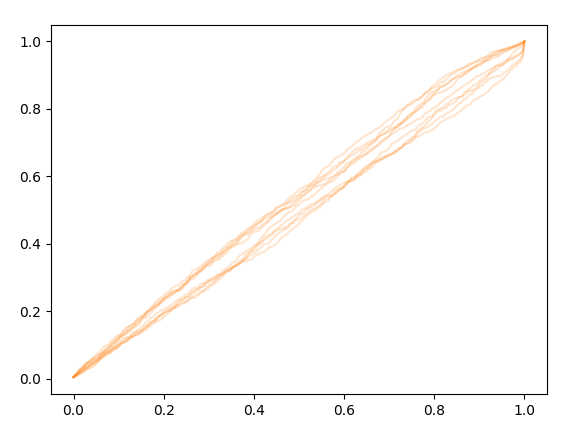
\includegraphics[width=0.99\linewidth]{figures/ppplot.pdf}
    \caption{Cumulative distribution of the quantile of which the true value
    lies for each marginalized distribution. The shadow band denotes the 95\%
    credible interval drawn from a uniform distribution with the same number of
    events as the injection campaign. The legend shows the p-values for each
    marginalized distribution.}
    \label{fig:ppplot}
    \end{figure}

\subsection{Real event parameter estimation}

To demonstrate the performance of our parameter estimation pipeline, we apply
it to two real LIGO-Virgo events: GW150914 and GW170817. We use the priors
shown in Table \ref{tab:parameters}, and take 4 s of data sampled at 2048 Hz
for the GW150914 analysis, and 128 s of data sampled at 4096 Hz for the
GW170817 analysis; strain data and PSDs for both events are fetched from GWOSC
\cite{GWOSC}. For our specific choice of sampler settings, we produce
${\sim}$2500 and 3500 \emph{effective samples}\footnote{Effective
samples here refers to the number of independent samples, which is the total
number of generated samples divided by their correlation length; we compute the
effective sample size using
\textsc{arviz},\url{https://python.arviz.org/en/stable/api/generated/arviz.ess.html}.
\cite{arviz_2019}} for GW150914 and GW170817 respectively. Running on an Nvidia A100
GPU, the wall time for both events is around 10 minutes. Most of this
time is spent on just-in-time (JIT) compilation of the code; the actual
sampling time is only ${\sim}150$ s. We pre-compute the reference waveform
parameters used in hetetrodyne likelihood for the two events, the time for
which is omitted in the \texttt{wall} time calculation.  The chain data and the
analysis scripts which generate the chains can be found in
%\kw{\variable{data/} and \variable{script}}
.

\begin{figure}
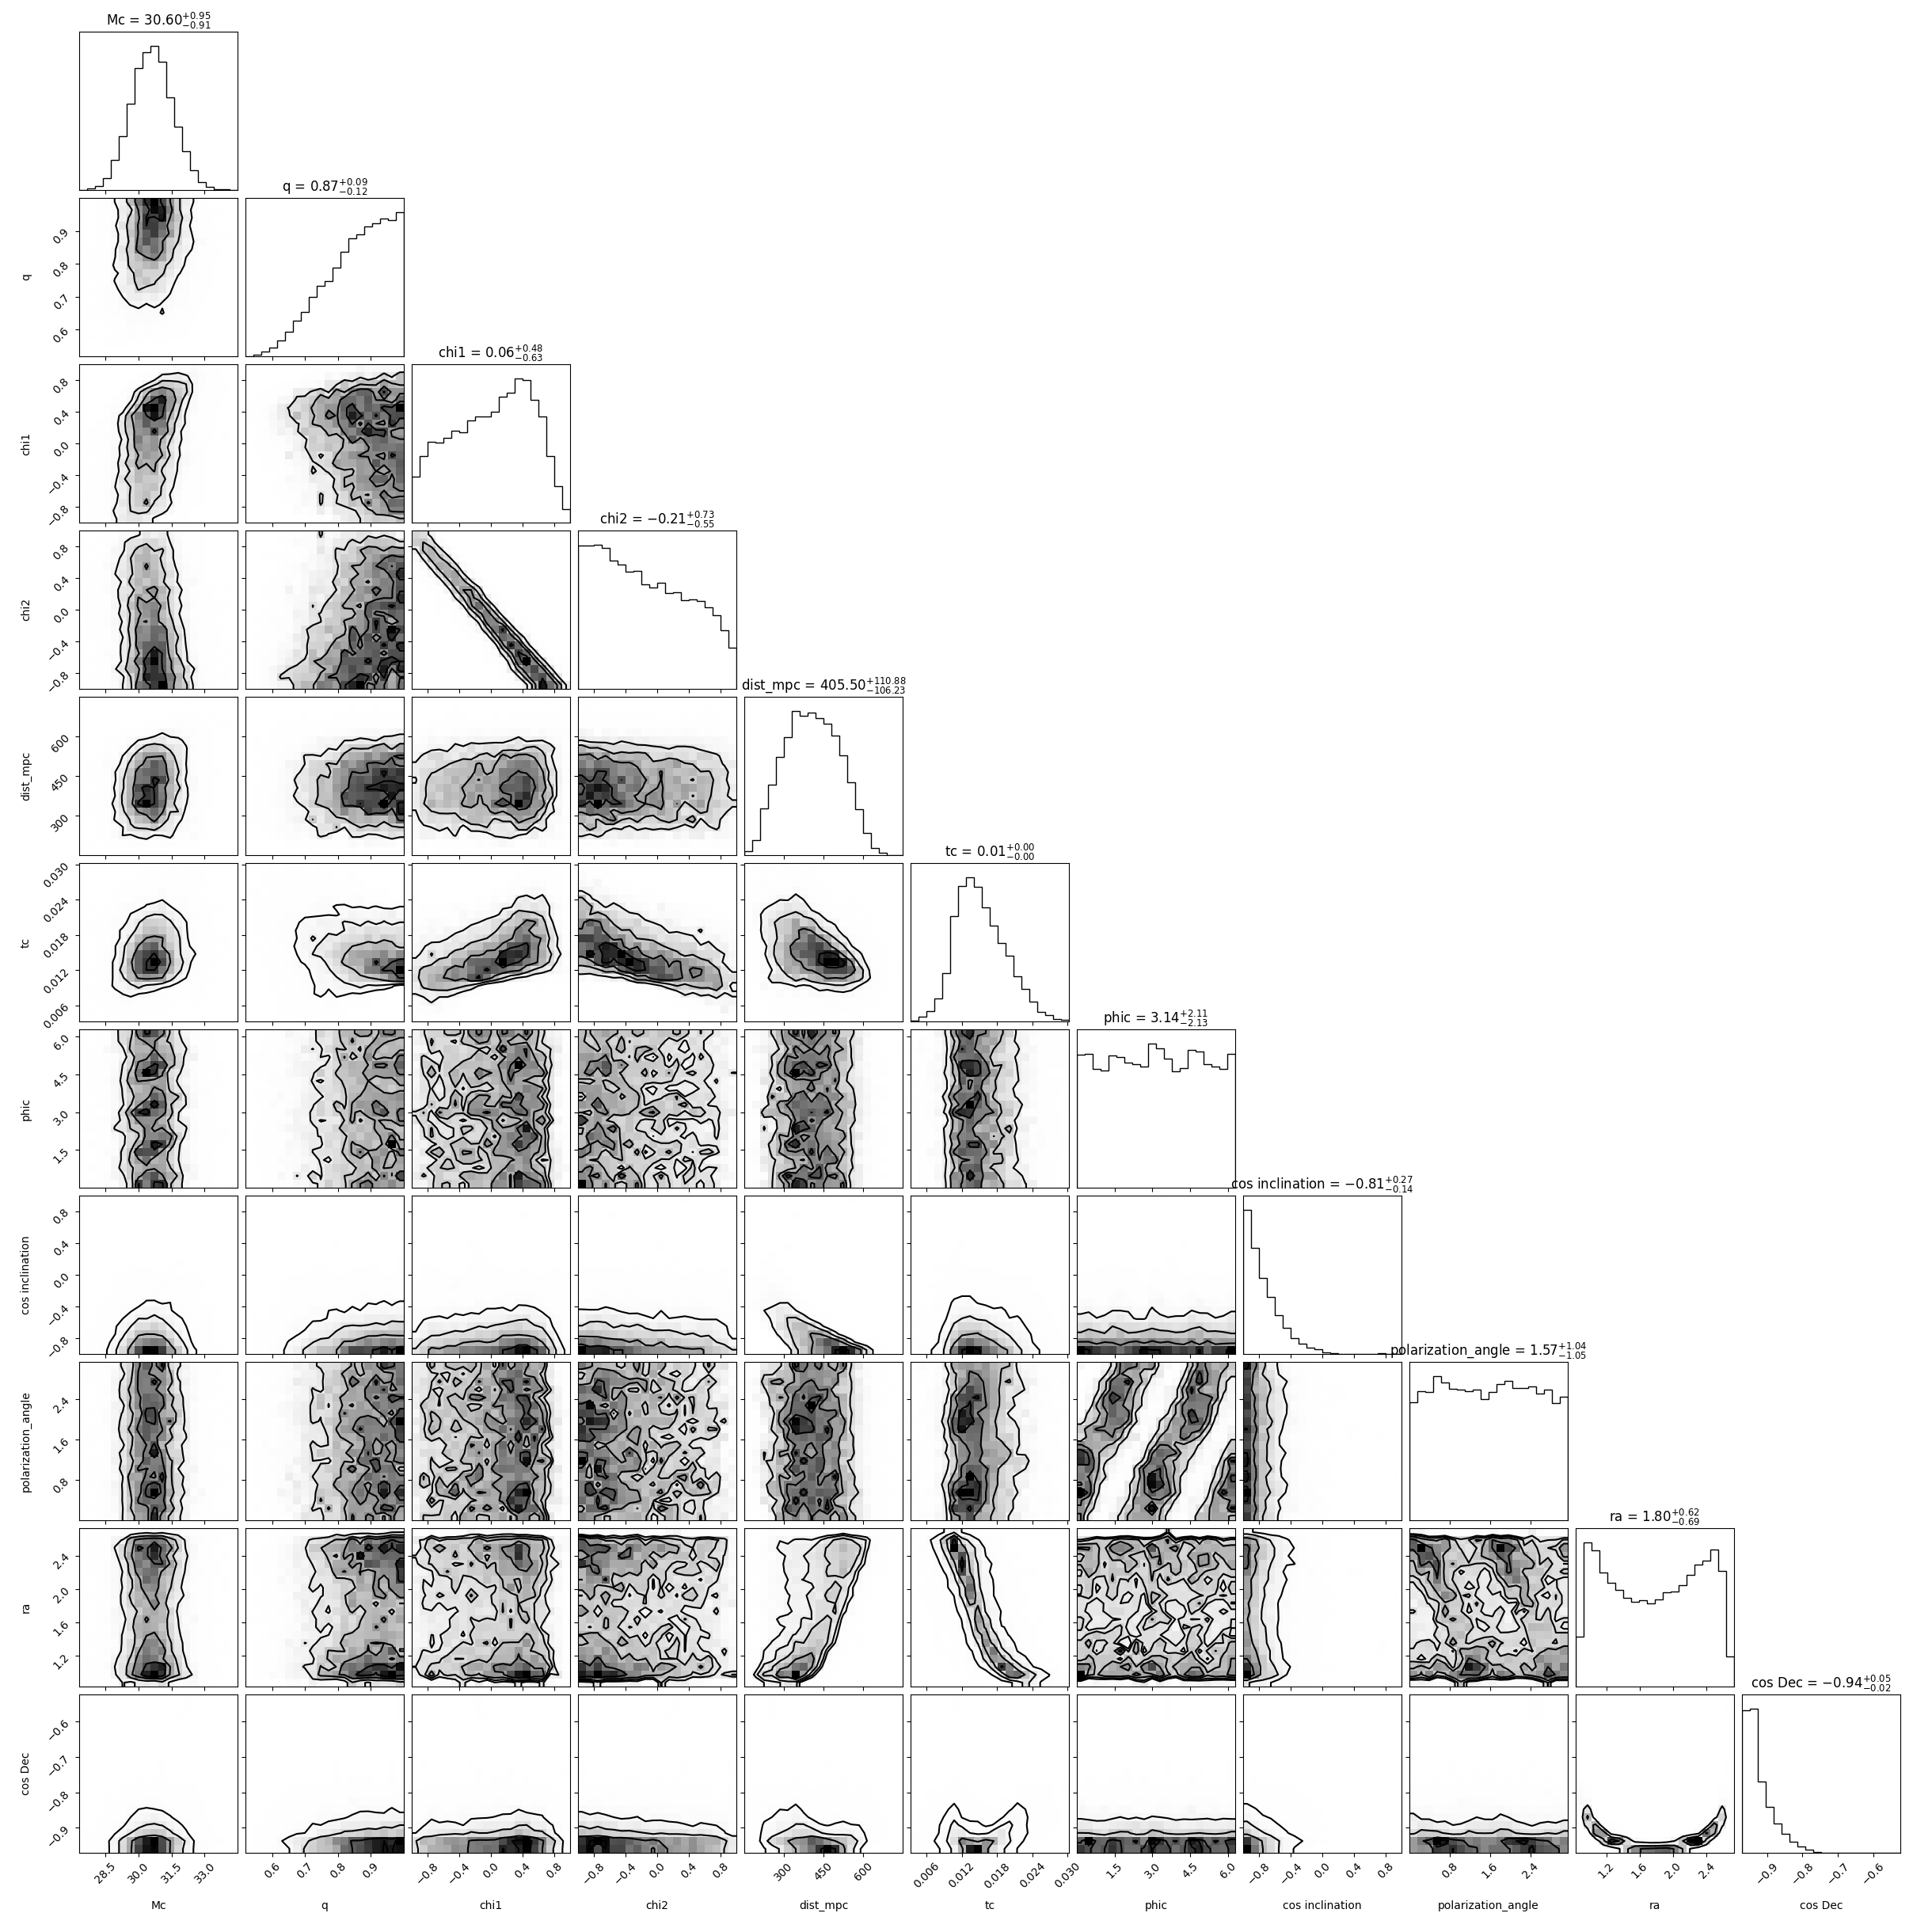
\includegraphics[width=0.99\linewidth]{static/GW150914.png}
\caption{
    GW150914 posterior computed by our code (blue) and \textsc{Bilby} (orange).
}
\label{fig:GW150914}
\end{figure}

\begin{figure}
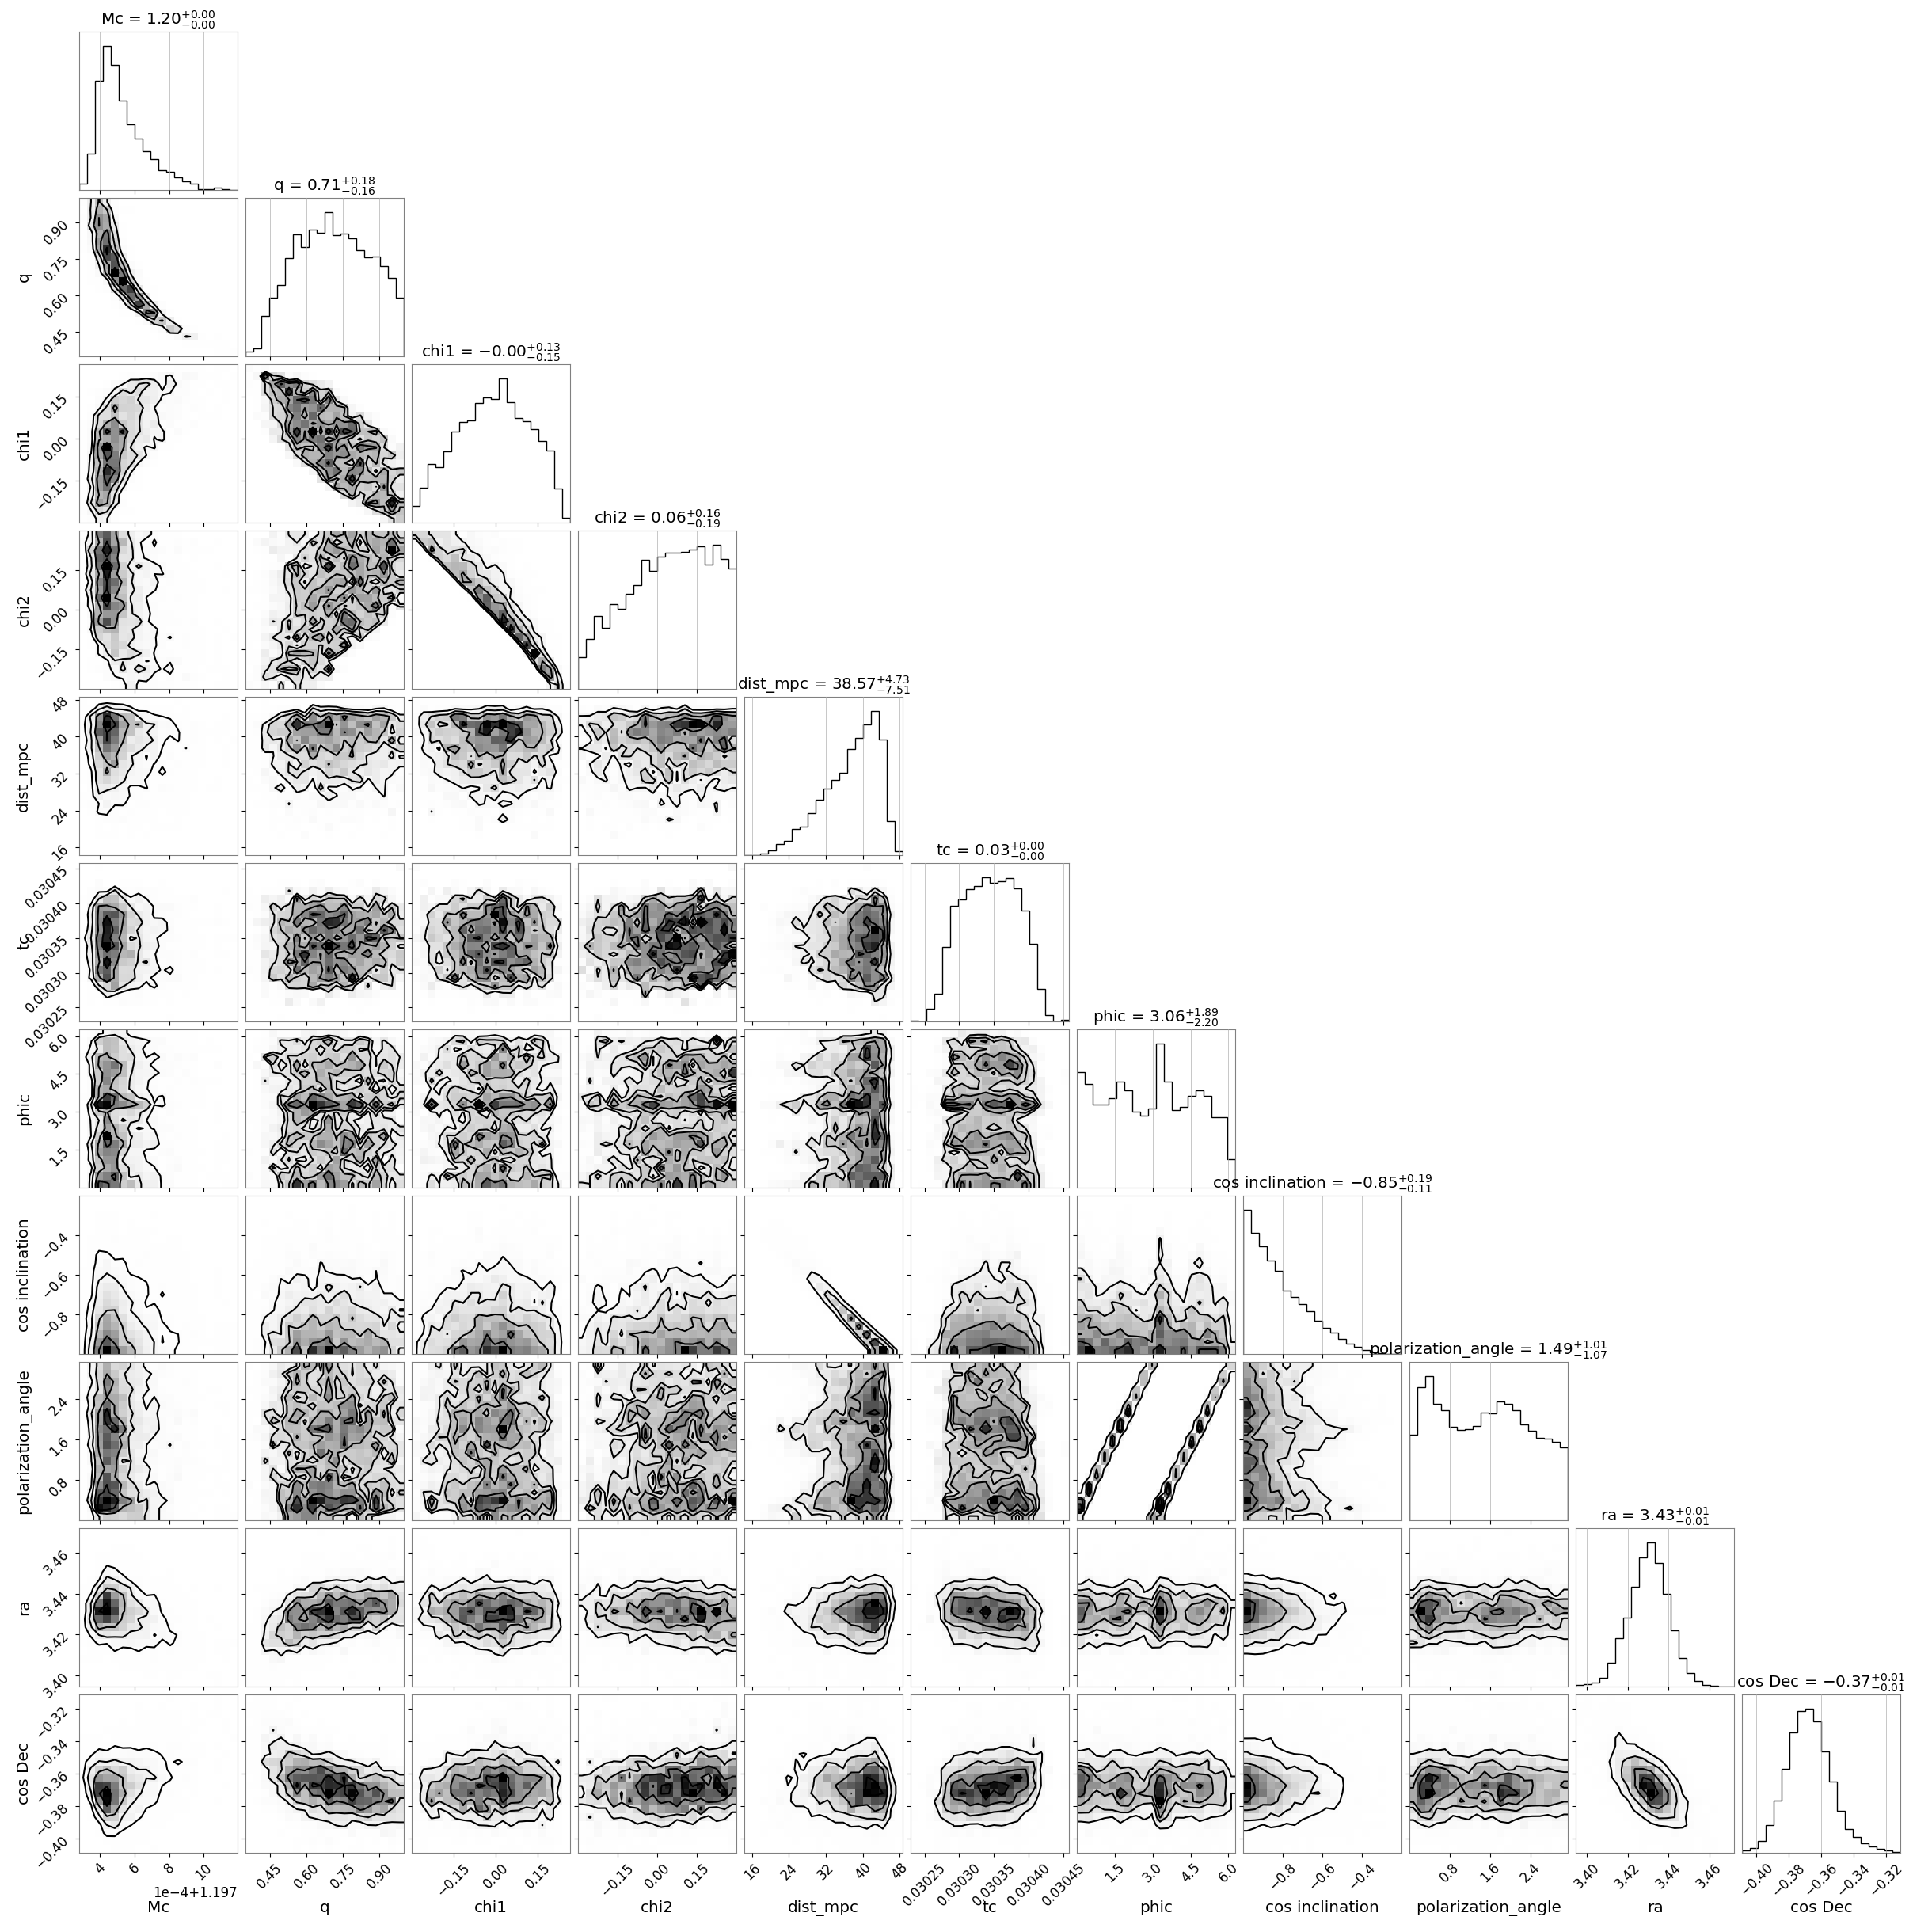
\includegraphics[width=0.99\linewidth]{static/GW170817.png}
\caption{
    GW170817 posterior computed by our code (blue) and \textsc{Bilby} (orange).
}
\label{fig:GW170817}
\end{figure}

For comparison, we produce equivalent runs with \textsc{Bilby}, using the same
exact data and priors.  We use the \textsc{dynesty} sampler
\cite{2020MNRAS.493.3132S,dynesty}, with 1000 live points and other settings as
shown in \cite{release}.  We carry out these runs using \textsc{parallel Bilby}
(\textsc{pBilby}) \cite{Smith:2019ucc} to distribute the computation over 400
Intel Skylake CPUs for each event.  For the specific settings chosen, the
wall-time duration of each run is ${\sim}1$ day for GW150914 and ${\sim}2$ days
for GW170817.

% Describe the distance between flowMC result and Bilby result using
% Jensen-Shannon divergence, scipy has a function to compute that in
% scipy.spatial.distance

Figs.~\ref{fig:GW150914} and \ref{fig:GW170817} show that our posteriors are
consistent with those produced by \textsc{Bilby}.  For a quantitative
comparison, we compute the Jensen-Shannon divergence between our code and
\textsc{Bilby} for the marginalized distribution for each parameter. The
Jensen-Shannon divergence is a symmetric measure of the distance between two
probability distributions, with a value of 0 indicating identical distributions
and a value of $\ln{2} \textrm{nat}$ representing the maximum possible
divergence between two distributions.

\kw{Report JSO} 

\section{Discussion}
\label{sec: Discussion}

% Brief summary
In this work, we present a PE pipeline for GW events that is efficient and
flexible. Our package put together a number of innovations, including
differentiable waveform models from \texttt{ripple} \kw{cite}, heterodyned
likelihood and normalizing flow enhanced sampler \texttt{flowMC}. We tested the
robustness of our pipeline on a set of 1200 synthetic GW events, showing it is
capable of handling catalogs that will be available in the near future. We also
demonstrate our pipeline can estimate the parameters of GW150914 and GW170817 in
\kw{Quote speed}. 

% Compared to other works
There are recent works from different groups on speeding up parameter
estimation of gravitational wave, including efficient reparameterization
\cite{Islam:2022afg,Roulet:2022kot} and deep learning
\cite{Dax:2021tsq,Dax:2022pxd}. While all of these methods can get down to
minutes-scale parameter estimation with high fidelity, our approach possesses
unique strengths, and may complement some of those other techniques.

% Stephen's work
Compared to \cite{Dax:2021tsq,Dax:2022pxd}, we do not rely on pre-training the neural
network on a large collection of waveforms and noise realization. This means as
soon as new waveform models and noise models are available, our algorithm can
already be deployed. Furthermore, our method is essentially an MCMC algorithm,
which inherits the merit of convergence measures in MCMC. As we are only using
the normalizing flow as a proposal distribution, and the normalizing flow is
trained jointly with a local sampler, we do not suffer from overfitting since
our training data is being generated on the fly and is always approaching the
target distribution. In this sense, we do not introduce potential extra
systematic error to inference results.

While our pipeline uses the sample generated by the local sampler for training,
one can also supply a pre-trained normalizing flow model to our pipeline to
bypass the training stage. This can further reduce the total runtime of our
inference pipeline. However, this may introduce potential systematic bias in the
inference result if the pre-trained network is not able to capture the
complexity presented in the data.

%Tousif's work
Compared to \cite{Islam:2022afg,Roulet:2022kot}, we do not rely on handcrafted
reparameterization of the coordinate systems. If the reparameterization scheme
is known ahead of time, a nice reparameterization is also encouraged. However,
handcrafted reparameterization depends on the assumptions used in deriving the
reparameterization scheme, which would inevitably run into limitations of use
cases. Our work can be viewed as an automatic reparameterization powered by
normalizing flow, while not being exact hence as efficient as an explicit
reparameterization, the method proposed in this work applies to a much border
class of problems, such as parameter estimation with precessing waveforms,
testing GR, and multi-event joint inference.

It is always beneficial to reparameterize if the reparameterization is known
ahead of time. For the class of problems where
\cite{Islam:2022afg,Roulet:2022kot} applies, we can incorporate the
reparameterization scheme into our MCMC pipeline to reduce the complexity of the
problem, hence speeding up the training phase. On the other hand, if there is
part of the target posterior that is not included in the reparameterization
scheme, the normalizing flow should still be able to learn to produce accurate
samples efficiently.

The two relevant works represent two orthogonal directions one can take in
building next generation tools in general. On one hand, there are modern tools
such as deep learning that are very flexible and powerful, but may need to rely
on having highly robust training data. On the other hand, there are traditional
tools that make use of our understanding of the underlying physics to simplify
the problem, which relies on having good intuition of the problem. Both
approaches rely on having a somewhat reasonable prior on how to approach the
problem. The main difference between methods used in industrial products and
scientific problems is scientific problems often try to address questions one
may have not been answered before, hence it is supposed to be far away from our
prior knowledge, meaning one need to take capability to generalize beyond the
current problem into account while building the tool. Our work utilizes both
reparameterization and deep learning, yet our method can be trivially extended
to problems beyond standard GW analysis that reparameterization or deep learning
alone may have trouble dealing with. We believe such flexibility is crucial for
building scientific tools.

% Additional traits for having differentiable waveforms
There are some future developments we are working on. While IMRPhenomD
\cite{Khan:2015jqa} is a reasonable start, it lacks some qualitative features
that other state-of-the-art models have, such as precession, higher mode, and
eccentricity. It also has a higher mismatch with reference numerical relativity
waveforms compared to more recent waveform models. Currently, we are working on
building differentiable IMRPhenomPv2 \cite{Khan:2018fmp} and three-parameters
NRSurrogate waveforms \cite{Varma:2018mmi}. Going forward, we encourage the
waveform development community to leverage autodiff environments such as Jax
when constructing new waveform models. Having a differentiable waveform model is
not only beneficial for parameter estimation, but also for other applications
such as calibrating waveforms to numerical relativity results, as detailed in
\kw{cite}.

% Access to higher dimensional problem
While standard GW analysis goes up to 17 dimensions. non-standard GW PE problems
can have more parameters, which could potentially lead to more complicated
geometry in the target posterior that is hard to reparameterize. For example,
\cite{LIGOScientific:2021sio} introduces 10 extra parameters to modify the
post-Newtonian coefficients predicted in GR, which should be taken care at the
same time during inference. On top of the increase of dimensionality, these
parameters often introduce non-trivial degeneracies such as local correlation
and multi-modality. Therefore, currently testing GR is limited to varying these
modifications one at a time, partially due to the bottleneck in the sampler.
Given the gradient-based and normalizing flow-enhanced sampler, our code shows
the potential in solving this problem in full at once.

% Other detectors configuration

To perform realistic PE with our pipeline, the antenna pattern of the
detector network needed to be taken into account. Our current code can perform
parameter estimation for any combination of the Hanford, Livingston, and Virgo
detectors, under the assumption of short signals such that the effect of Earth's
rotation can be ignored. For next-generation detector networks such as the
Einstein Telescope and the Cosmic Explorer, a differentiable version
of their antenna pattern is needed.

% More features such as marginalization
The features we have implemented are the barebone version of parameter
estimation. We do not include marginalization schemes such as time, phase, and
calibration lines marginalization \cite{2019PASA...36...10T}. Because of the reasonable performance of the
sampler on accelerators, time and phase marginalization is not necessary, as the
performance of our implementation is not significantly impacted by having two
extra dimensions. Nevertheless, having less parameters in a PE is always
appreciated, which we are looking into including in our code as well as other
marginalization modes.

% JIT overhead
Jax's JIT compilation drastically reduces the computational time to evaluate the
likelihood. However, it comes with a compilation overhead when the likelihood is
evaluated for the first time. We observe that the compilation time could depend
on the device where the code will be run. This is expected since Jax leverage
Accelerated Linear Algebra (XLA) takes advantage of accelerators, which means
Jax needs to compile the code for the specific device according to its
architecture. On an Nvidia A100 GPU, the compilation overhead could go up to 8
minutes for the waveform we are using. For the cases we have studied, the time
needed to obtain converging results on an A100 is about 2-3 minutes. This means
the compilation overhead is dominating the wall-clock time of the specific PE
run we considered. To utilize our implementation to its full potential, we are
looking into ways to reduce the compilation overhead or to cache the
compilation results to avoid paying the compilation overhead for every event.

% Faster maximum likelihood finder

Another overhead we are looking into reducing is the time needed to find the
reference waveform for heterodyning the likelihood. Currently, we are using
\texttt{differential evolution} \cite{Storn1997DifferentialE} available in
\texttt{scipy} to find the waveform parameters which maximize the likelihood.
Since \texttt{differnetial evolution} has not been implemented in Jax, and the
Jax waveform we use is not compatible with the parallelization scheme in the
\texttt{scipy} library, it takes around 5 minutes \kw{Benchmark it in the code
and make this number precise.} to find the reference waveform parameters for
GW170817. There are two ways to improve the performance in finding the
parameters of the reference waveform. First, we can explore different
optimization strategy that is more compatible with the strength of our pipeline,
in particular differentiability of our likelihood and the possibility to
evaluate many waveforms in parallel with a GPU. Particle swarm \cite{7869491}
and stochastic gradient descent methods \cite{10.5555/304710.304720} are
promising candidates which we intend to investigate in the future. 

Another way to reduce the time of finding the maximum likelihood waveform is to
incorporate marginalization of extrinsic parameters to reduce the dimensionality
of the optimization problem. Currently, we simultaneously maximize all 11 GW
parameters, which is unnecessarily complicated and expensive. There are
long-existing marginalization schemes over extrinsic parameters such as the merger
time and phase, which can find the corresponding maximum likelihood waveform
much more efficiently when compared to differential evolution. We expect
implementing these marginalization schemes will reduce the time needed to find
the reference waveform parameters by obtaining the extrinsic parameters and by
reducing the dimensionality of the optimization problem for the intrinsic
parameters.

% Multi-device scaling
One important aspect of modern computing is scalability, meaning it is generally
favorable if one can simply put more computing units in the same problem and
reduce the Wall time. In our case, this means we would like to use more than one
GPU for the same PE process. More GPUs can help in the following ways: first,
more GPUs means we can run more independent chains at the same time, which can
generate more samples faster. But more importantly, as shown in this work and
\kw{cite flowMC?}, more independent chains also help with reducing the burn-in
time. Parallelizing over the number of chain dimension is trivial and does not
require much change to the current infrastructure. Another way more GPUs can
helps is by allowing faster training of larger flow models. While the training time
is not the biggest bottleneck given the flow model used in this study, more GPUs
means we can increase the bandwidth of the flow model by increasing its size
while keeping the training time the same. This helps capture more complex
geometry in the target space, which can lead to more accurate results in general.


\section{Acknowledgements}
Thanks Will.

\bibliography{bib}

\end{document}
